% ============================================
% SECCIÓN 1: Motivación
% ============================================
\section{Motivación}

\begin{frame}{El problema: Medir la geometría de los poros}
    \begin{columns}[T]
        \column{0.5\textwidth}

        \begin{block}{Material: AAO}
            Membrana nanoestructurada con poros cilíndricos organizados en red hexagonal. Sus propiedades ópticas y mecánicas dependen de la geometría de los poros.
        \end{block}

        \begin{block}{Objetivo}
            Predecir automáticamente los parámetros geométricos de una imagen SEM.
        \end{block}

        \begin{alertblock}{5 variables objetivo}
            \renewcommand{\arraystretch}{1.25}
            \begin{tabular}{@{}ll@{}}
              $R$,\;$\sigma_R$       & Radio promedio y dispersión [px] \\
              $DCC$,\;$\sigma_{DCC}$ & Distancia centro a centro [px] \\
              $P$                    & Porosidad (\%) \\
            \end{tabular}
        \end{alertblock}

        \column{0.5\textwidth}

        \begin{center}
            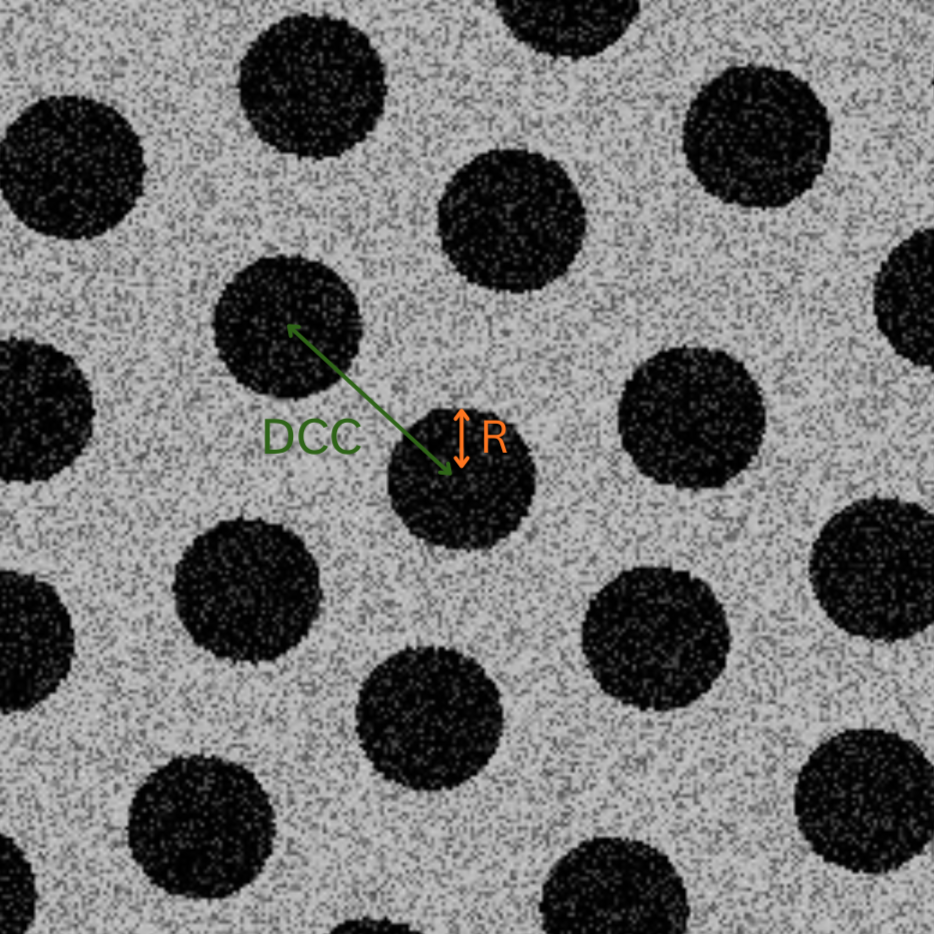
\includegraphics[width=0.7\textwidth]{chapters/introduction/ImagenAAO.png}
        \end{center}

    \end{columns}
\end{frame}
